\section{A Simplified Model for Shear Flow}
\begin{frame}{A Simplified Model for a Two-Dimensional Flow}
	\scriptsize
	For a two-dimensional flow on $S^2$, i.e. $\boldsymbol{n} :=(\sin \theta \cos \phi, \sin \theta \sin \phi, -\cos \theta)^T$ with $\theta \in (0,\pi)$ and $\phi \in (0, 2\pi)$, we define
	$\boldsymbol{u} = \left( 0, 0, w(x,y, t)\right)^T$.\\
	\vspace{0.4cm}
	\pause
\textcolor{blue}{Drift Diffusion term} 
   \begin{align*}
   \partial_{t}\left(\sin \theta f\right) +\partial_\theta\left(( w_x \sin^3 \theta \cos \phi \cos - w_y\sin \phi \sin^3 \theta) f\right) =D_{r}(\partial_{\theta\theta}\partial_{\phi\phi})f
   \end{align*}
\textcolor{red}{Spatial transport term}
\begin{align*}
	\nabla_x \cdot ((I+n \otimes n)e_3f) =  -\partial_x((\cos\phi \sin\theta \cos\theta)f) - \partial_y((\sin\phi \sin \theta \cos \theta)f).
\end{align*}
\pause
Assuming $\gamma = 0$, we get:
\begin{align*}
	&\partial_{t}\left(\sin \theta f\right)+ \textcolor{blue}{\partial_\theta\left(( w_x \sin^3 \theta \cos \phi + w_y\sin \phi \sin^3 \theta) f\right)}\\
	&+\textcolor{red}{\partial_x(\cos\phi \sin\theta \cos\theta f)} + \textcolor{red}{\partial_y(\sin \phi \sin \theta \cos \theta f)}
	= \textcolor{blue}{D_{r}(\partial_{\theta\theta}\partial_{\phi\phi})f}. \\
	&Re\partial_{t}w = \partial_{xx}w + \partial_{yy}w + \delta(\bar{\rho}-\rho(x,t))
\end{align*}
\end{frame}


\begin{frame}
	\scriptsize
	\begin{figure}[H]
		\centering
		\begin{minipage}{0.4\textwidth}
			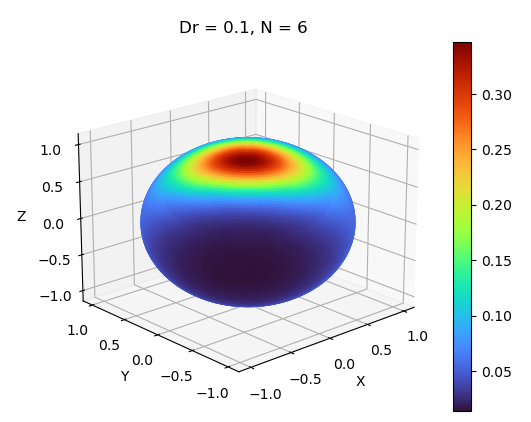
\includegraphics[scale=0.4]{Bilder_wxwy/Sol_onSphere_wxwy_Dr=0.1_N=6}
		\end{minipage}
		\hfill 
		\begin{minipage}{0.4\textwidth}
			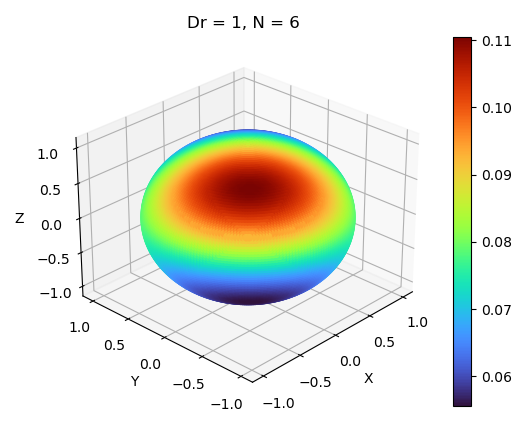
\includegraphics[scale=0.4]{Bilder_wxwy/Sol_onSphere_wxwy_Dr=1_N=6}
		\end{minipage}
		\caption{ Numerical solution of the drift-diffusion term with constant externally imposed velocity gradient corresponding to shear flow using different values of $D_r$ and $N = 6$.}
	\end{figure}
\end{frame}


\begin{frame}{A Simplified Model for a One-Dimensional Flow}
	\scriptsize
For a one-dimensional flow we assume $	\boldsymbol{u} = (0,0,w(x,t))^T$. \\
\vspace{5mm}
\textcolor{blue}{Drift Diffusion term} 
    \begin{align*}
	\partial_{t}\left(\sin \theta f\right)+ \partial_\theta\left(w_x \sin ^3 \theta \cos \phi f\right)
	=D_{r}(\partial_{\theta\theta}\partial_{\phi\phi})f.
    \end{align*}
\textcolor{red}{Spatial transport term}
   \begin{align*}
   	\nabla_x \cdot ((I+n \otimes n)e_3f) =\partial_x( -\cos\phi \sin\theta \cos\theta)f.
   \end{align*}
 	Assuming $\gamma = 0$, we have:
 \begin{align*}
 	&\partial_{t}\left(\sin \theta f\right)+ \textcolor{blue}{\partial_\theta\left(w_x \sin ^3 \theta \cos \phi f\right)} - \textcolor{red}{\partial_x(-\cos\phi  \cos\theta \sin\theta^2f)}
 	= \textcolor{blue}{D_{r}(\partial_{\theta\theta}\partial_{\phi\phi})f}, \\
 	&Re\partial_{x}w = \partial_{xx}w + \delta(\bar{\rho}-\rho(x,t)).
 \end{align*}
\end{frame}

\begin{frame}
	\scriptsize
	\begin{figure}[H]
		\centering
		\begin{minipage}{0.4\textwidth}
			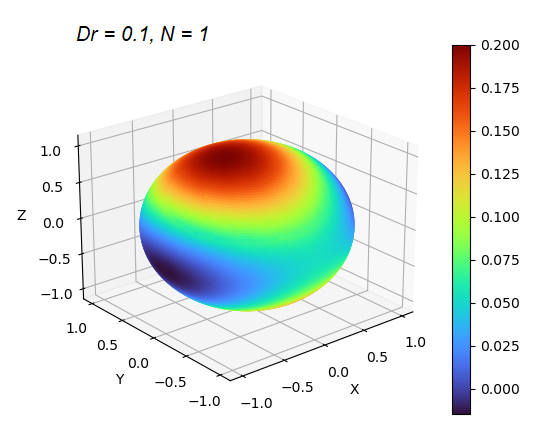
\includegraphics[scale=0.4]{Bilder_wx/wx=1_Dr=0.1_N=1}
		\end{minipage}
		\hfill 
		\begin{minipage}{0.4\textwidth}
			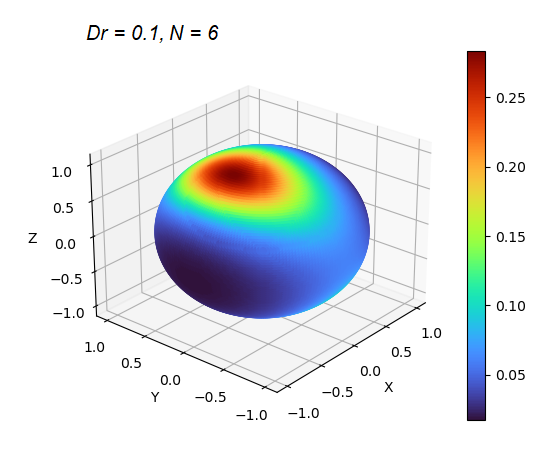
\includegraphics[scale=0.4]{Bilder_wx/wx=1_Dr=0.1_N=6}
		\end{minipage}
	    \hfill 
	    \begin{minipage}{0.4\textwidth}
		  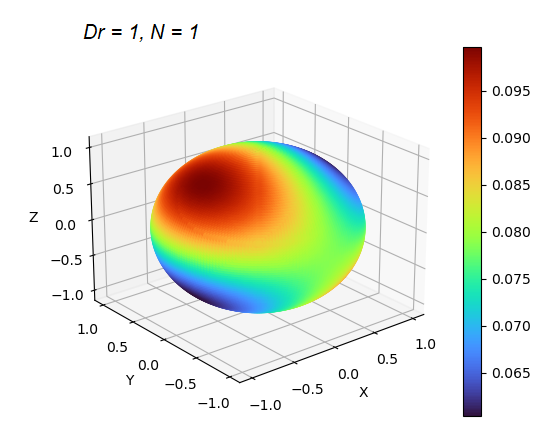
\includegraphics[scale=0.4]{Bilder_wx/wx=1_Dr=1_N=1}
	    \end{minipage}
         \hfill 
        \begin{minipage}{0.4\textwidth}
	      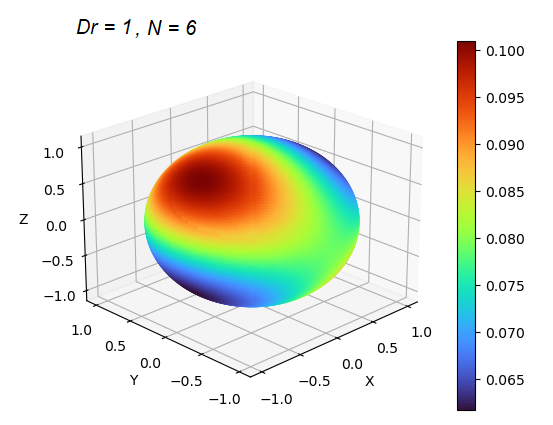
\includegraphics[scale=0.4]{Bilder_wx/wx=1_Dr=1_N=6}
        \end{minipage}
		\caption{ Numerical solution of the drift-diffusion term with constant externally imposed velocity gradient corresponding to shear flow using different values of $D_r$ and $N = 1,6$.}
	\end{figure}
\end{frame}

